% ===== 9. Чому цифровий тренер =====
\newcommand{\argcard}[2]{%
  \begin{tcolorbox}[colframe=accent,colback=accent!6,boxrule=0.6pt,arc=2pt,
    height=2.55cm,valign=top,left=5pt,right=5pt,top=4pt,bottom=4pt]
    \raggedright\textbf{#1}\par\smallskip
    \small #2
  \end{tcolorbox}}

\begin{frame}{Чому цифровий тренер}
  \begin{columns}[T,onlytextwidth]
    \begin{column}{0.49\textwidth}
      \argcard{Працює з тим, що в пілота вже є}
        {Камера чи телефон, а не Garmin Catalyst 2 за \$1,199.99}
      \argcard{Люди готові платити за тренування}
        {Живий тренер — €250–350 на день, Track Titan залучив \$5 млн}
    \end{column}
    \begin{column}{0.49\textwidth}
      \argcard{Дані відкриті й належать пілоту}
        {Формат GPMF у відеофайлі, без API чи дозволу компаній}
      \argcard{Поради, а не графіки}
        {2–3 поради з цифрами й відео для новачка}
    \end{column}
  \end{columns}

  \note{[Доповідач 3] Чому саме цифровий тренер? Перше: він працює з тим, що в пілота вже є, — з камерою чи телефоном, а не з пристроєм на кшталт Garmin Catalyst 2 за \$1,199.99. Друге: дані відкриті. GoPro пише телеметрію у форматі GPMF прямо у відеофайл, і цей файл належить пілоту. Нам не потрібен дозвіл чи API жодної компанії — на відміну від кошика. Третє: люди вже платять за тренування. Живий тренер коштує €250–350 на день, а Track Titan залучив \$5 млн. І четверте: ми закриваємо проміжок між графіками і дорогими пристроями — даємо новачку дві-три поради з цифрами і відео.}
\end{frame}

% ===== 10. Як виглядатиме продукт =====
\begin{frame}{Як виглядатиме продукт}
  \begin{columns}[c,onlytextwidth]
    \begin{column}{0.62\textwidth}
      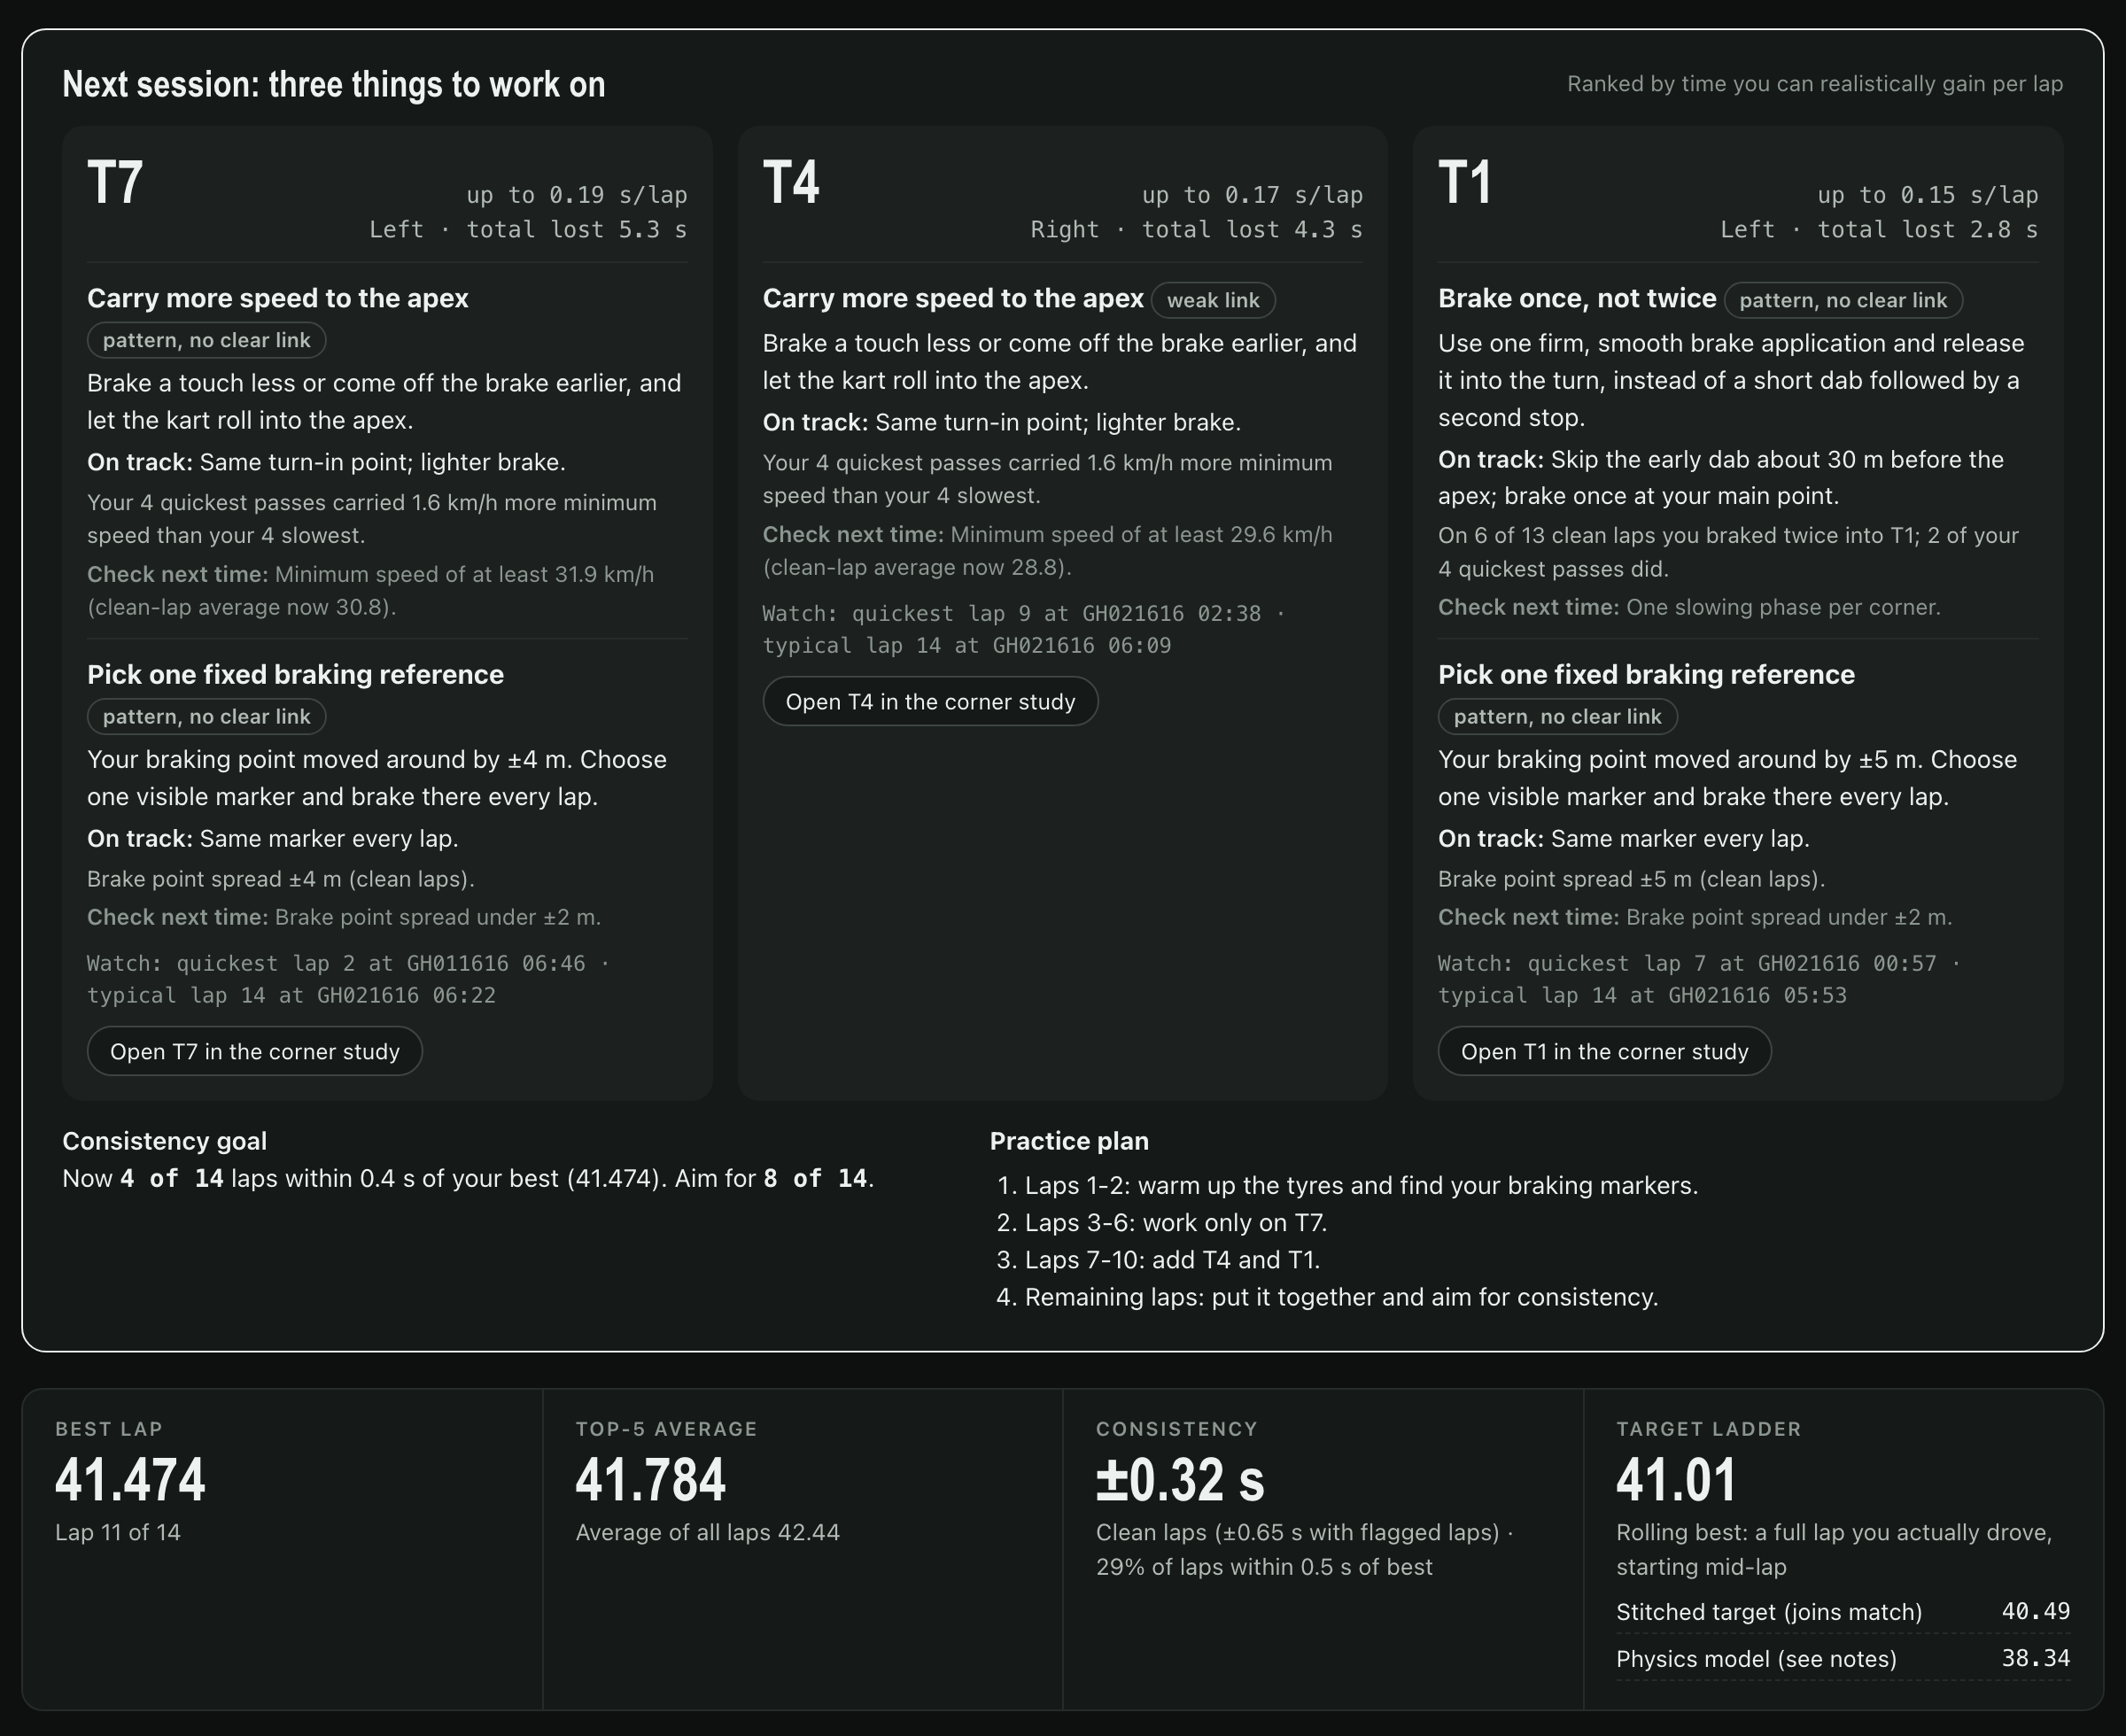
\includegraphics[width=\linewidth,height=0.82\textheight,keepaspectratio]{img/session-debrief.png}
    \end{column}
    \begin{column}{0.35\textwidth}
      \begin{itemize}
        \item Реальна сесія: 14 кіл, «Жага швидкості», GoPro HERO7
        \item Три повороти з порадами й планом на наступний заїзд
        \item Біля кожної поради — момент у відео
      \end{itemize}
    \end{column}
  \end{columns}

  \note{[Доповідач 4] Ось як це виглядатиме. Це макет розбору однієї реальної сесії: 14 кіл на картодромі «Жага швидкості», знято на GoPro HERO7. Угорі — блок «три речі, над якими працювати»: повороти, де можна виграти найбільше часу. Для кожного є порада простими словами і цифра, яку варто перевірити наступного разу, а також посилання на момент у відео. Нижче — план на наступний заїзд і підсумкові цифри сесії. У повному макеті є ще карта траси з межами і таблиця часу по колах. Саме такий результат пілот має отримувати після кожного заїзду.}
\end{frame}

% ===== 11. Ризики =====
\begin{frame}{Ризики і як ми з ними працюємо}
  \centering
  \begin{tabularx}{\textwidth}{@{}>{\raggedright\arraybackslash}p{0.38\textwidth} >{\raggedright\arraybackslash}X@{}}
    \toprule
    \textbf{Ризик зі SWOT} & \textbf{Що робимо в проєкті} \\
    \midrule
    Точність GPS у телефоні \textasciitilde{}4,9 м (W1)
      & Основне джерело — GoPro з GPS, телефон — з попередженням \\
    Точні межі траси потребують фото з дрона (W6)
      & Межі із супутника, невпевнені ділянки — пунктиром \\
    Криті картодроми без GPS (W3)
      & MVP — лише відкриті траси \\
    Tenth Finder і Kart Track уже дають поради (T1)
      & Перевіряємо їх до розробки; ми — без нового обладнання \\
    \bottomrule
  \end{tabularx}

  \note{[Доповідач 4] Звісно, ризики є, і ми їх не ховаємо. Точність GPS у телефоні — близько 4,9 метра. Тому основним джерелом буде відео GoPro з GPS, а трек із телефона підтримаємо з попередженням про точність. Точні межі траси потребують фото з дрона, тож у MVP беремо межі із супутникових знімків, а невпевнені ділянки показуємо пунктиром і порад щодо траєкторії там не даємо. Криті картодроми без GPS у MVP не входять. А конкурентів, Tenth Finder і Kart Track, ми встановимо й перевіримо ще до розробки. Повний список ризиків і рішень є в документі з рішенням.}
\end{frame}
